\documentclass[tikz]{standalone}

\colorlet{FilledSurface}{blue!20}
\colorlet{FilledSurfaceGroupOne}{blue!20}
\colorlet{FilledSurfaceGroupTwo}{red!20}
\colorlet{FilledSurfaceGroupThree}{green!20}
\colorlet{FilledSurfaceGroupFour}{magenta!20}
\colorlet{FormulaBackground}{green!10}
\colorlet{FormulaFrame}{green}


\usetikzlibrary{calc, intersections, decorations.markings}

\tikzset{
    mark rect/.style={
        decoration={markings, mark=at position 0.5 with {
            \draw[fill=white] (-6pt,-2pt) rectangle (6pt,2pt);
        }}, postaction={decorate}
    }
}

\begin{document}
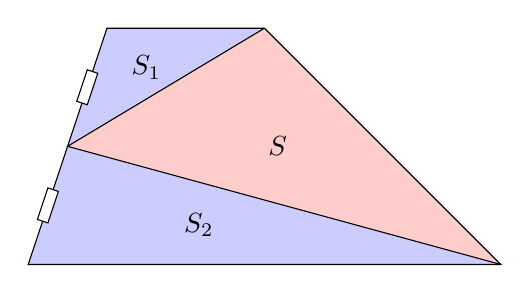
\begin{tikzpicture}

\coordinate (A) at (0, 0);
\coordinate (B) at (1, 3);
\coordinate (C) at (3, 3);
\coordinate (D) at (6, 0);

\coordinate (M) at ($(A)!0.5!(B)$);

% Colorear superficies
\fill[FilledSurfaceGroupOne] (B) -- (M) -- (C);
\fill[FilledSurfaceGroupOne] (A) -- (D) -- (M);
\fill[FilledSurfaceGroupTwo] (C) -- (D) -- (M);

\node at (barycentric cs:B=1,M=1,C=1) {$S_1$};
\node at (barycentric cs:M=1,A=1,D=1) {$S_2$};
\node at (barycentric cs:C=1,M=1,D=1) {$S$};

% Dibujamos los segmentos, luego de colorear las superficies para
% evitar que las superficies cubran a los segmentos.
\draw (A) -- (B) -- (C) -- (D) -- cycle;
\draw (D) -- (M) -- (C);

\path[mark rect] (A) -- (M);
\path[mark rect] (B) -- (M);

\end{tikzpicture}
\end{document}
